\documentclass[tikz,border=3mm]{standalone}
\usepackage{fontspec}
\usepackage{amsmath}
\usepackage{xcolor}
\usepackage{tikz}
\usetikzlibrary{
  arrows.meta,
  backgrounds,
  calc,
  decorations.pathreplacing,
  fit,
  positioning,
  shapes.geometric,
  shapes.symbols
}

\IfFontExistsTF{Comic Sans MS}
  {\setmainfont{Comic Sans MS}}
  {\setmainfont{TeX Gyre Heros}}

\tikzset{
  >={Stealth[length=2.2mm,width=1.6mm]},
  figure title/.style={font=\fontsize{14}{16}\selectfont,align=center},
  figure subtitle/.style={font=\fontsize{8}{10}\selectfont,align=center},
  figure label/.style={font=\fontsize{7.5}{9}\selectfont,align=center},
  figure tiny/.style={font=\fontsize{6.2}{7.4}\selectfont,align=center},
  data flow/.style={-Stealth,line width=1.0pt},
  control flow/.style={-Stealth,dashed,line width=.8pt},
  projection/.style={densely dotted,line width=.8pt},
  compute/.style={rectangle,rounded corners=1.6mm,line width=.8pt,
    minimum height=.72cm,inner xsep=5pt,inner ysep=3pt,figure label},
  event/.style={diamond,aspect=1.3,line width=.8pt,inner sep=1.4pt,figure tiny},
  store/.style={cylinder,shape border rotate=90,aspect=.28,line width=.8pt,
    minimum height=.78cm,figure label},
  state/.style={circle,line width=.8pt,minimum size=.72cm,figure tiny},
  fusion/.style={regular polygon,regular polygon sides=6,line width=.8pt,
    minimum width=1.4cm,figure tiny}
}

\definecolor{accent}{HTML}{0B6B45}
\definecolor{accentdark}{HTML}{06452E}
\definecolor{ink}{HTML}{18342B}
\definecolor{graphite}{HTML}{3F5D53}
\definecolor{pale}{HTML}{E7F5EE}
\definecolor{paper}{HTML}{FBFCF7}
\definecolor{divider}{HTML}{B9D2C8}
\definecolor{secondary}{HTML}{087F8C}
\definecolor{highlight}{HTML}{F2A900}


\begin{document}
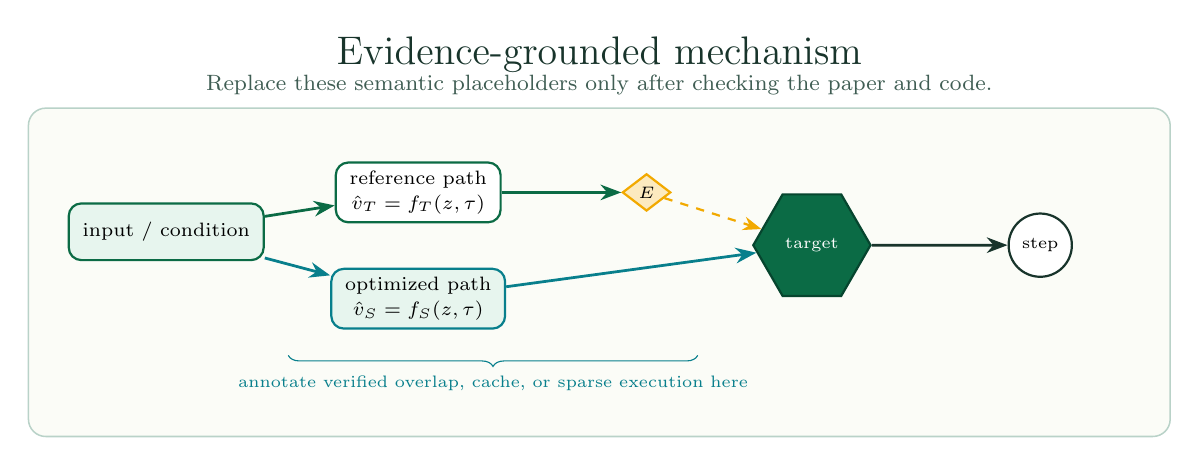
\begin{tikzpicture}[x=1cm,y=1cm]
  \node[figure title,text=ink] at (7.5,5.2) {Evidence-grounded mechanism};
  \node[figure subtitle,text=graphite] at (7.5,4.82)
    {Replace these semantic placeholders only after checking the paper and code.};

  \fill[rounded corners=2.2mm,fill=paper,draw=divider,line width=.55pt]
    (.25,.35) rectangle (14.75,4.52);

  \node[compute,fill=pale,draw=accent] (input) at (2.0,2.95)
    {input / condition};
  \node[compute,fill=white,draw=accent] (teacher) at (5.2,3.45)
    {reference path\\$\hat v_T=f_T(z,\tau)$};
  \node[compute,fill=pale,draw=secondary] (student) at (5.2,2.10)
    {optimized path\\$\hat v_S=f_S(z,\tau)$};
  \node[event,fill=highlight!25,draw=highlight] (event) at (8.1,3.45)
    {$E$};
  \node[fusion,fill=accent,draw=accentdark,text=white] (merge) at (10.2,2.78)
    {target};
  \node[state,fill=white,draw=ink] (step) at (13.1,2.78)
    {step};

  \draw[data flow,draw=accent] (input) -- (teacher);
  \draw[data flow,draw=secondary] (input) -- (student);
  \draw[data flow,draw=accent] (teacher) -- (event);
  \draw[control flow,draw=highlight] (event) -- (merge);
  \draw[data flow,draw=secondary] (student) -- (merge);
  \draw[data flow,draw=ink] (merge) -- (step);

  \draw[decorate,decoration={brace,mirror,amplitude=4pt},draw=secondary]
    (3.55,1.38) -- (8.75,1.38);
  \node[figure tiny,text=secondary] at (6.15,1.02)
    {annotate verified overlap, cache, or sparse execution here};
\end{tikzpicture}
\end{document}
